
\documentclass[useAMS,usenatbib]{mn2e}
\pdfminorversion=4
\usepackage{bm}
\usepackage{graphicx}

%\renewcommand\includegraphics[2][]{}
\nonstopmode

\newcounter{ionstage}
\newcommand{\ion}[2]{\setcounter{ionstage}{#2}% 
  \ensuremath{\mathrm{#1\,\scriptstyle\Roman{ionstage}}}}
\newcommand\nii{[\ion{N}{2}]}
\newcommand\sii{[\ion{S}{2}]}
\newcommand\oiii{[\ion{O}{3}]}
\newcommand\ha{\ensuremath{\mathrm{H\alpha}}}
\newcommand\hii{\ion{H}{2}}

%% New macros that are needed for version 2 of the MS
\newcommand\gammaVCAthin{\ensuremath{\gamma_{\mathrm{t}}}}
\newcommand\gammaVCAvthick{\ensuremath{\gamma_{\mathrm{T}}}}
\newcommand\mSF{\ensuremath{m_{\mathrm{2D}}}}
\newcommand\mSFddd{\ensuremath{m_{\mathrm{3D}}}}

\begin{document}

\setcounter{section}{2}\setcounter{subsection}{3}\setcounter{subsubsection}{2}
\subsubsection{Velocity channel analysis}
\label{sec:stats-vca} %% New label for sec 2.3.3


\setcounter{figure}{5}
\setcounter{section}{3}\setcounter{subsection}{2}\setcounter{subsubsection}{1}
\subsubsection{Second-order Structure Functions}
\label{sssec:s2func}
\begin{figure*}
  \centering
  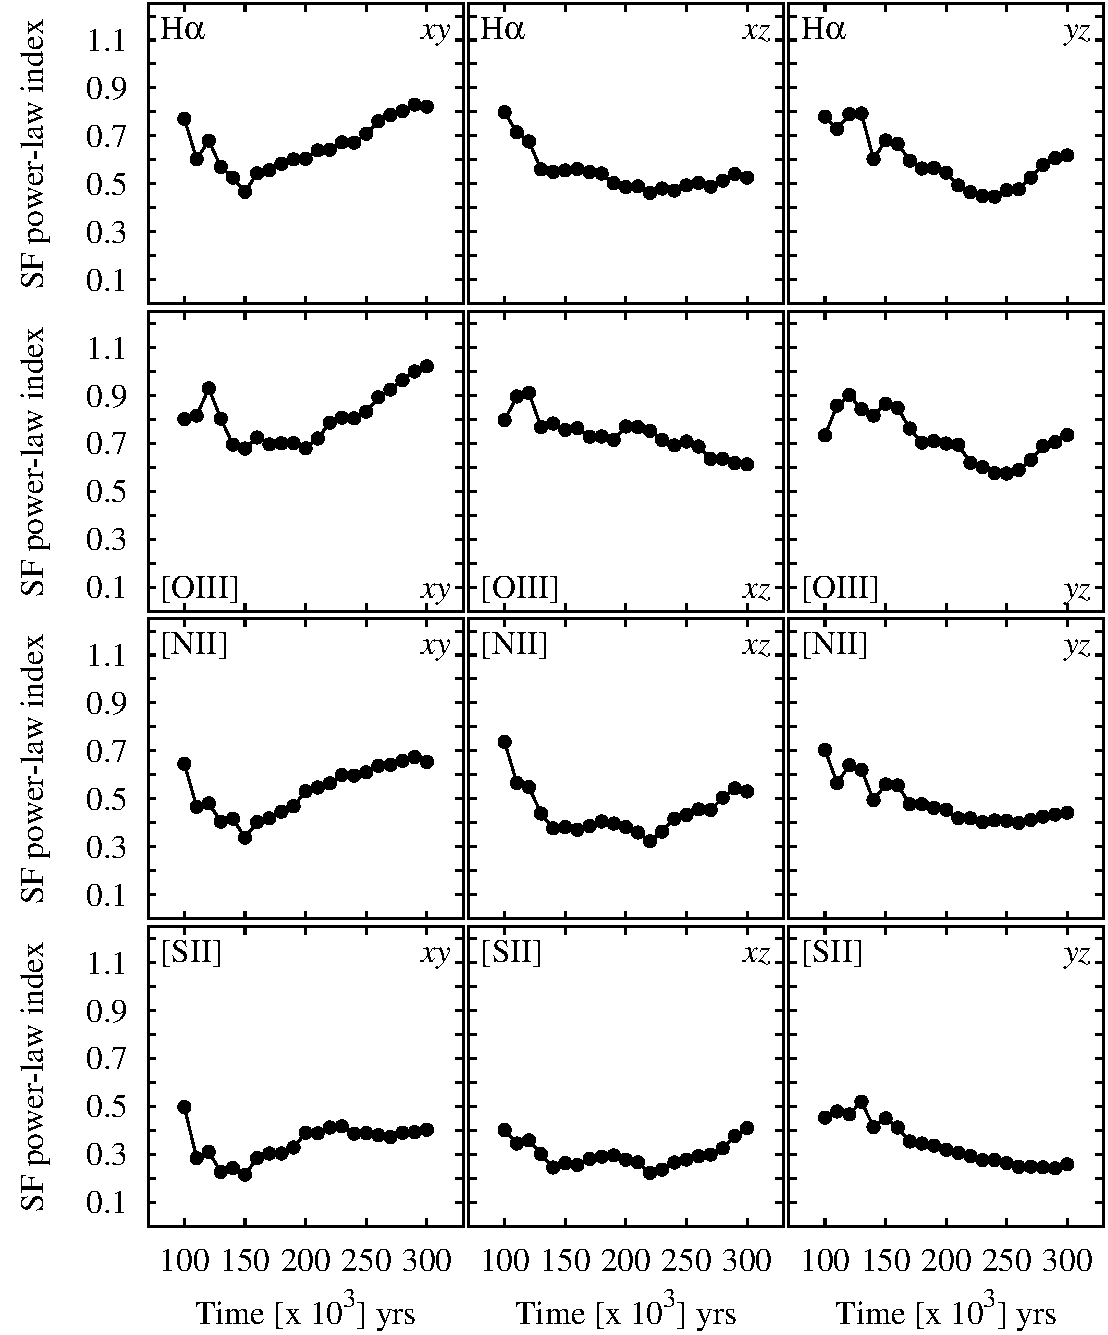
\includegraphics[width=\textwidth]{sf-time-trends-all}
  \caption{Evolution of second-order structure function power-law
    index, \mSF, as a function of time. From top to bottom: H$\alpha$,
    \oiii{} $\lambda 5007$, \nii{} $\lambda 6584$, \sii{} $\lambda
    6716$. From left to right: line of sight along the $z$, $x$ and
    $y$ axes, respectively.}
  \label{fig:sftrends}
\end{figure*}

\begin{figure*}
\centering
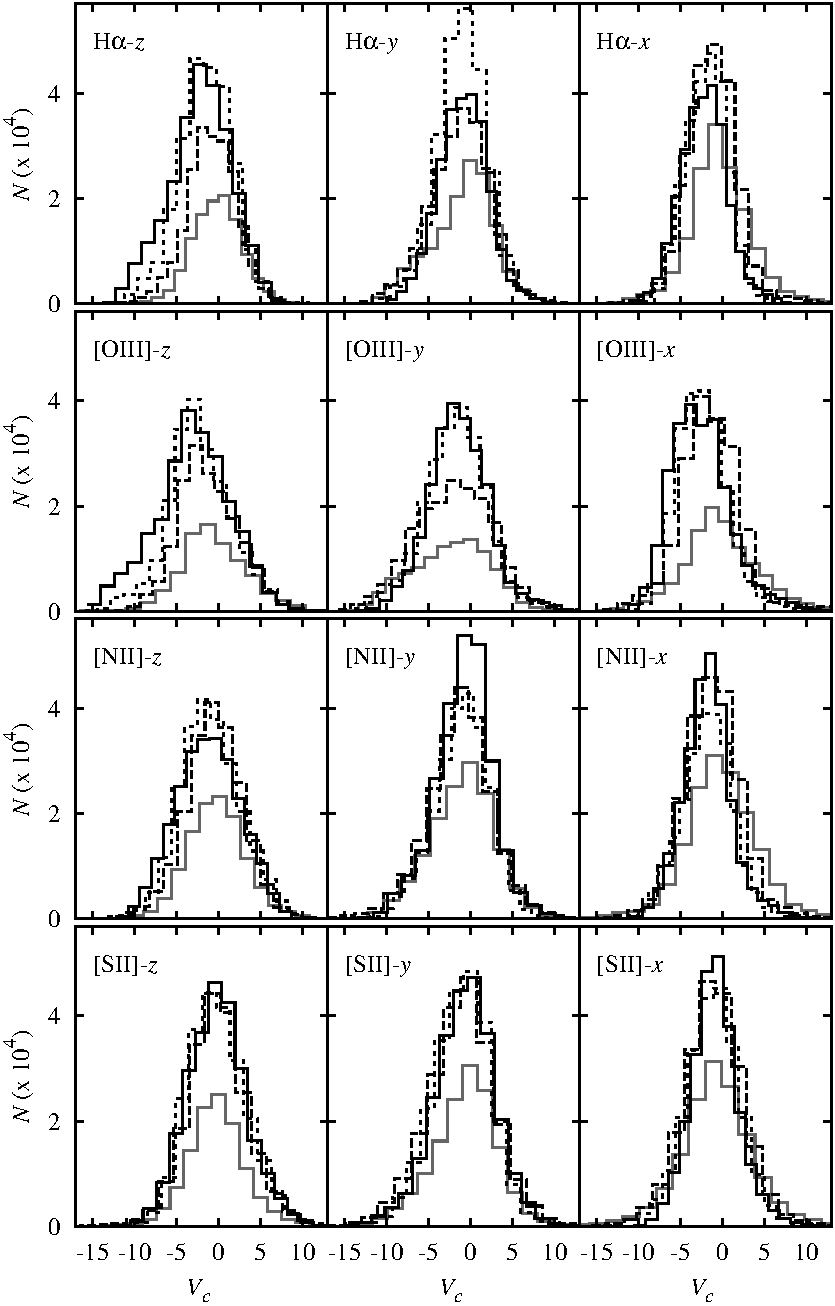
\includegraphics[width=0.6\linewidth]{pdf-centroid}
\caption{Histograms of velocity centroid values for each emission line
  along different lines of sight. From top to bottom: H$\alpha$,
  \oiii$\lambda 5007$, \nii$\lambda 6584$, \sii$\lambda 6716$. From
  left to right: line of sight along the $z$, $x$ and $y$ axes,
  respectively. The different line types refer to different times:
  thick, grey line---150,000~yrs, dashed line---200,000~yrs,
  short-dashed line---250,000~yrs, continuous black
  line---300,000~yrs.}
\label{fig:histogram}
\end{figure*}

We use the procedure described in Section~\ref{subsubsec:centroid} to
calculate velocity centroid maps for the H$\alpha$, \oiii$\lambda
5007$, \nii$\lambda 6584$ and also \sii$\lambda 6716$ emission lines
and then calculate the corresponding second-order structure functions
according to Equation~\ref{eq:strucfunc}. Results for representative
evolutionary times are shown in Figures~\ref{fig:sfunc} to
\ref{fig:sfuncyz} of Appendix~\ref{app:sf}, where power law fits to
the slope (\mSF) of the structure function are carried out for the
inertial range of scales.

In Figure~\ref{fig:sftrends} we show the evolution of \mSF{} with time
for the different lines and for the three principal viewing directions
of the simulation cube.  For the line of sight along the $z$-axis
(first column of Fig.~\ref{fig:sftrends}), one sees for all lines a
consistent steepening of the structure function graph with time
(increase in \mSF{}).  But for other viewing directions no such trend
is apparent: both rising and falling behavior of \mSF{} is seen, with
little consistency between different lines.

In order to understand why one particular viewing direction is
different, we produced histograms of the emission-line velocity
centroid values binned into narrow $<2$~km~s$^{-1}$ bins for the three
different lines of sight at the four different times. The histograms
are presented in Figure~\ref{fig:histogram}, from which we see that
for the $z$-axis line of sight, the values of $V_c$ are not
distributed symmetrically about the mean value and, in fact, for the
H$\alpha$ and \oiii$\lambda$5007 emission lines, a ``wing'' develops
for negative values of $V_c$ that extends to more negative values as
time progresses. This tendency is not seen for the $y$- and $x$- axis
lines of sight. We attribute this wing to a ``champagne'' flow towards
the observer along the $z$-axis. This flow would be perpendicular to
the line of sight for observations along the other axes.



%% WJH 25 Jul 2014 - Table of struc func indices removed


\subsubsection{Velocity Channel Analysis}
\label{sssec:vca}
\begin{figure*}
%% Figure 8 in ms-resubmit.pdf
\centering
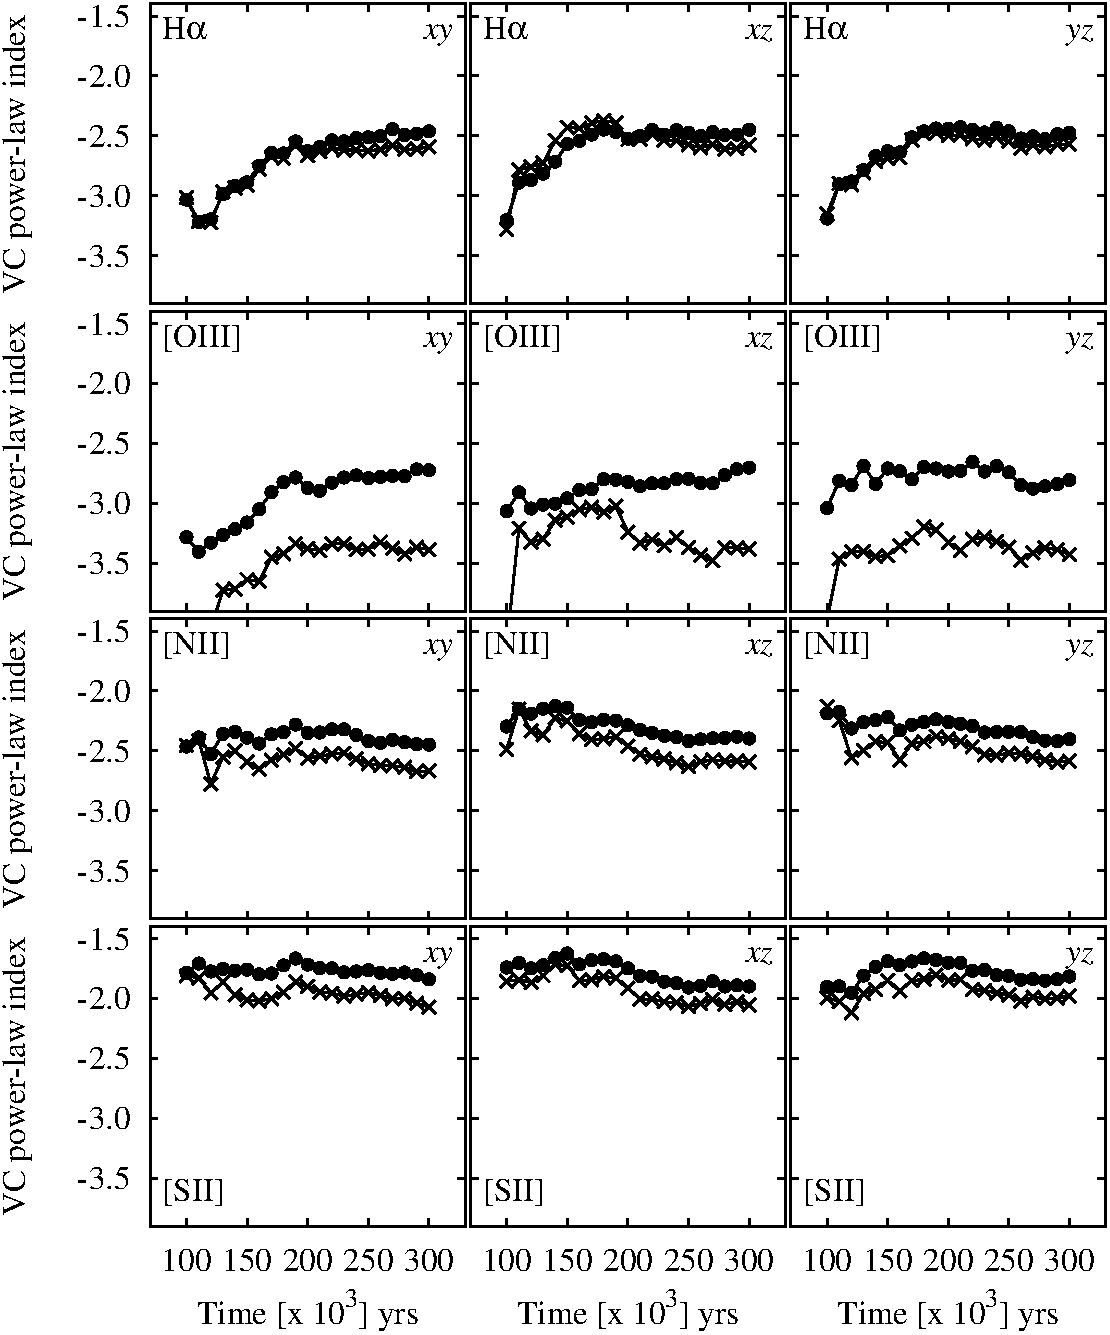
\includegraphics[width=\textwidth]{vca-time-trends-all}
\caption{ Evolution of velocity channel power-law index as a function
  of time for thick channels (\gammaVCAvthick; crosses) and thin
  channels (\gammaVCAthin; filled circles).  From top to bottom:
  H$\alpha$, \oiii{} $\lambda 5007$, \nii{} $\lambda 6584$, \sii{}
  $\lambda 6716$. From left to right: line of sight along the $z$, $x$
  and $y$ axes, respectively.  Thermal broadening was included in all
  cases.  }
\label{fig:vcatrends}
\end{figure*}

Figure~\ref{fig:vcatrends} shows the evolution with time of the VCA
slope from thin and thick channels (shown by filled circle and cross
symbols, respectively) for different ions and for different viewing
directions.  The individual VCA power spectra from which these slopes
were extracted are presented in Appendix~\ref{app:vca}.  It can be
seen that both \gammaVCAthin{} and \gammaVCAvthick{} are remarkably
stable with time during the latter part of the evolution (\(t >
200,000\)~years).  Although thermal broadening means that there is no
clear distinction between \gammaVCAthin{} and \gammaVCAvthick{} for
the H\(\alpha\) line, the two values are clearly distinguished for the
heavier ions, with the thin slices showing a significantly shallower
slope, especially for \oiii{}.  The implications for diagnosing
turbulence statistics are discussed in \S~\ref{sssec:vca2}.


\setcounter{section}{4}\setcounter{subsection}{1}\setcounter{subsubsection}{1}
\subsubsection{Structure Function}
\label{sssec:strfunc}
The structure function of the velocity centroids is an observationally
attractive diagnostic because it is relatively immune to the effects
of thermal broadening and poor spectral resolution, so long as
sufficiently high signal-to-noise spectra are used.  However, it has
the disadvantage that relating the observed slope to the 3-dimensional
velocity statistics depends on the geometry of the emitting region,
see \S~\ref{subsec:projsmooth}.  For transverse separations larger
than the characteristic line-of-sight depth of the emitting gas, the
two-dimensional gradient should be equal to the three-dimensional one:
\[
m_{\mathrm{2D}} = m_{\mathrm{3D}} = -3 - n,
\]
whereas at smaller separations than this, 
projection smoothing, as described above, means that 
the two-dimensional gradient is steeper:
\[
m_{\mathrm{2D}} = 1 + m_{\mathrm{3D}} = -2 - n.
\]
Based on our simulation's velocity power spectrum index at late times
of \(n \approx -3.2\) (see Figs.~\ref{fig:ps} and \ref{fig:psevol}),
the structure function slope should be \(m_{\mathrm{2D}} = 0.2\) in
the large-scale limit and \(m_{\mathrm{2D}} = 1.2\) in the small-scale
limit.

In fact, all of the measured slopes lie between these two limits,
with a systematically increasing value from low to high-ionization lines:
\(m_{\mathrm{2D}}(\sii) = 0.45 \pm 0.01\), 
\(m_{\mathrm{2D}}(\nii) = 0.55 \pm 0.02\), 
\(m_{\mathrm{2D}}(\ha) = 0.60 \pm 0.03\), 
\(m_{\mathrm{2D}}(\oiii) = 0.75 \pm 0.03\). 
This is qualitatively consistent with expectations
because the emission from lower-ionization lines is confined to 
thin layers near the ionization front, whereas higher ionization emission
is more distributed over the volume
and therefore subject to greater projection smoothing.  

If the line-of-sight depth were constant over the face of the \hii{} region,
then the structure function would show a break at that scale,
but in reality the depth varies from point to point, 
so the break will be blurred out.
Instead, the structure function is expected to show negative curvature,
with the gradient gradually decreasing 
as one passes from smaller to larger scales. 
A small such effect is seen in the structure functions 
derived from our simulations (Fig.~\ref{fig:sfunc} to \ref{fig:sfuncyz}):
the fit to a power law is generally not so good as in the case of the power spectra,
with negative residuals at both ends of the fitted range,
indicative of a negative curvature.  
That the observed effect is so small is probably due to the fact that
the distribution of line-of-sight depths strongly overlaps with 
the limited dynamic range in separations available from our simulations,
bounded at small scales by numerical dissipation,
and at large scales by the size of the ionized region.

It is disappointing that none of the measured slopes
reach either of the limiting cases discussed above.
All that can be deduced from the structure function is that 
\(1 + m_{\mathrm{3D}} > m_{\mathrm{2D}}(\oiii)\) 
and \(m_{\mathrm{3D}} < m_{\mathrm{2D}}(\sii)\), which implies $n = -2.75$ to $-3.45$.
Although this is a rather wide range of allowed velocity power spectrum slopes,
it does serve to rule out the Kolmogorov value of \(n = -3.667\). 

A further proviso to the use of the structure function is that
systematic anisotropic flows can affect the measured slopes
when the viewing angle is along the direction of the flow.
Such an effect is seen at later times for our simulation
when viewed along the \(z\)-axis (Fig.~\ref{fig:sfunc}). 
In this case, the structure function tends to steepen
at the large-scale end of our fitting range,
producing a positive curvature, 
which is opposite to the more typical case of negative curvature discussed above.
Such cases may also be identified by the presence of a significant skew
in the PDF of the line-of-sight velocity (see Fig.~\ref{fig:histogram}).

Figure 

\begin{figure}
  \centering
  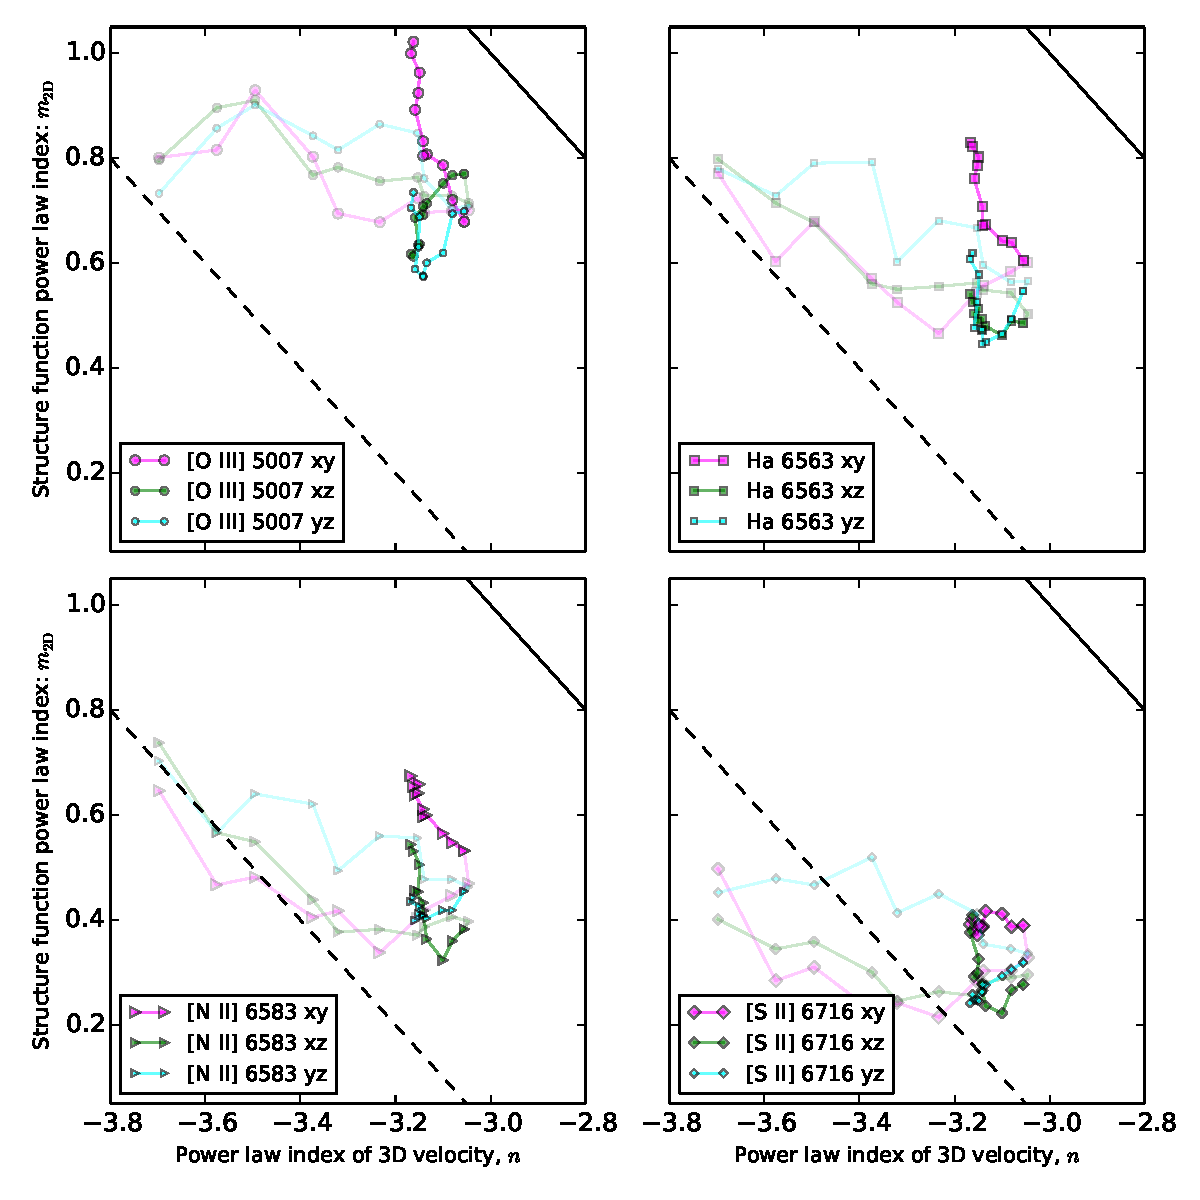
\includegraphics[width=\linewidth]{sf-vs-3d-panels}
  \caption{Structure function slope versus velocity power law slope}
  \label{fig:sf-vs-n}
\end{figure}

Note that the additional complication identified by \citet {2004ApJ...604..196B}, 
whereby correlations between density and velocity fluctuations affect the 
translation between \(m_{\mathrm{2D}}\) and \(n\), 
is likely of minor importance in our case.  
\citet {2007MNRAS.381.1733E} show that this is most important
for high Mach number turbulence, where \(\delta\rho/\langle \rho \rangle > 1\),
whereas the transonic turbulence inside our simulated \hii{} regions
produces more modest density contrasts. 
\begin{figure*}
\centering
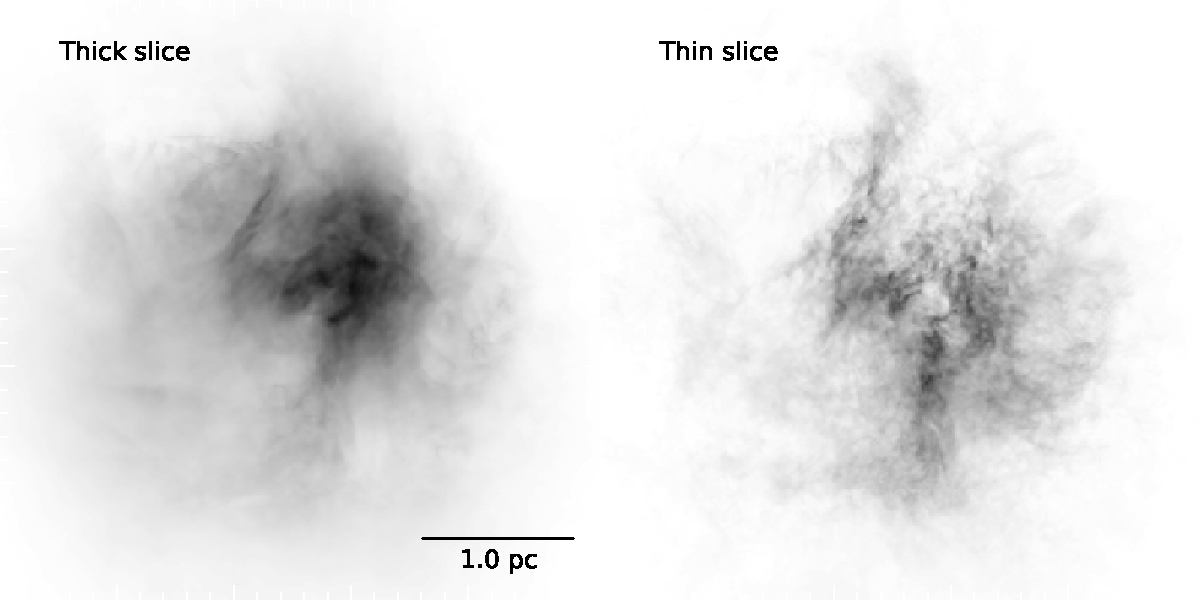
\includegraphics[width=\linewidth]{o3-thick-thin}
 \caption{Surface brightness maps in thick (left) versus thin (right) 
    velocity slices for the \oiii{} line from our simulation
    at an age of 300,000~years.  
    The thick slice covers the full velocity range of the emission line,
    while the thin slice has a width of 5~km~s$^{-1}$,
    which is smaller than the turbulent velocity fluctuations,
    but slightly larger than the thermal broadening for this line.
    It is apparent that the thin slice shows considerably greater
    small-scale structure than the thick slice,
    which is reflected in its shallower power spectrum.
    The brightness structure in the thick slice is due entirely to
    the emissivity fluctuations within the \hii{} region, 
    whereas the additional structure in the thin slice is caused by
    velocity fluctuations.
  }
\label{fig:o3-thick-thin}
\end{figure*}


\setcounter{section}{4}\setcounter{subsection}{1}\setcounter{subsubsection}{2}
\subsubsection{Velocity Channel Analysis}
\label{sssec:vca2}
The velocity channel analysis consists of calculating the
two-dimensional power spectrum of the brightness distribution
in isovelocity channels of varying thickness.  
We consider two cases: thick slices,
which are wide enough (\(\sim 100~\mathrm{km\ s^{-1}}\))
to include all the emission in the line,
and thin slices, with width \(5~\mathrm{km\ s^{-1}}\). 
Because the velocity spectrum in our simulations is rather shallow (see above),
the line-of-sight turbulent velocity dispersion \(\delta v\)
exceeds the width of these thin slices
over the full range of length scales that we can usefully study,
from \(0.1\)~pc (\(\delta v \approx 8~\mathrm{km\ s^{-1}}\))
to \(1\)~pc (\(\delta v \approx 10~\mathrm{km\
  s^{-1}}\)). Figure~\ref{fig:o3-thick-thin} shows typical examples of
the \oiii{} brightness in thick and thin slices.

To use thinner slices would not be useful for a variety of reasons.
First, \(5~\mathrm{km\ s^{-1}}\) corresponds to the highest resolution 
that can be achieved with optical spectrographs
that are optimised for studying extended sources,
such as Keck HIRES or VLT UVES. 
Second, thinner slices are increasingly subject to ``shot noise'' 
due to the finite resolution of the numerical simulations,
which produces spurious small-scale power, as discussed by 
\citet {2003MNRAS.342..325E} and \citet {2003ApJ...593..831M}.
Third, thermal broadening would smoothe out any structure on 
scales \(< 5~\mathrm{km\ s^{-1}}\) for all but the heaviest ions.

The procedure for deriving the power-law index
of the velocity fluctuations from the velocity channels is
slightly different, depending on whether the power spectrum 
of the emissivity fluctuations is ``steep'' or ``shallow'' (see above). 
In the steep case, which applies to \oiii{} in our simulation, 
the slope of the average power spectrum of the brightness maps
in the thin isovelocity channels is given by 
\(\gamma_{\mathrm{thin}} = -3 + \frac12 m_{\mathrm{3D}}\),
where \(m_{\mathrm{3D}} = -3 - n = 0.2 \pm 0.1\) for our simulation.
The derived value from the \oiii{} thin channel maps is 
\(\gamma_{\mathrm{thin}} = -2.84 \pm 0.11 \),
which compares very well with the value \(-2.9 \pm 0.05\)
that is implied by the simulation's value of \(n\). 

In the shallow case, it is the difference in slope
between the thin and thick slices
that is predicted to depend on the velocity fluctuations:
\(\gamma_{\mathrm{thin}} - \gamma_{\mathrm{vthick}} = \frac12 m_{\mathrm{3D}}\). 
The derived values are 
\(\gamma_{\mathrm{thin}} - \gamma_{\mathrm{vthick}} = 0.08 \pm 0.04\), 
\(0.18 \pm 0.04\), and \(0.18 \pm 0.04\)
for \ha, \nii, and \sii, respectively. 
These also compare well with the value of \(0.1 \pm 0.05\)
that is implied by the simulation's value of \(n\). 

The slopes of the power spectra of the thick slices themselves, 
which are simply the velocity-integrated surface brightness images\footnote{
  Although for simplicity, extinction is not included.}
are predicted \citep {2000ApJ...537..720L}
to be equal to the slopes of the 3D power spectra of their respective emissivities. 
However, only in the case of \oiii{} do we find this to be the case.
In the case of the other lines, \(\gamma_{\mathrm{vthick}}\) is shallower than
the emissivity's spectral index \(n\) by 0.36, 0.19, 0.61 for \ha, \nii, and \sii, respectively. 
The reason for this discrepancy may be the increasingly ``sheet-like'' morphology
of the emission in the lower ionization lines. 
As shown in \S~4.1 of \citet {2003ApJ...593..831M}, 
one should see a transition from \(\gamma_{\mathrm{vthick}} = n\) to the 
shallower slope \(\gamma_{\mathrm{vthick}} = n + 1\) at transverse scales larger
than the line-of-sight depth of the emitting region.



\appendix
\section[]{Example second-order structure functions of the line-of-sight velocity centroids}
\label{app:sf}
Figures~\ref{fig:sfunc} to \ref{fig:sfuncyz} show the second-order
structure functions of the line-of-sight velocity centroid maps (see
\S\S~\ref{sssec:strfunc} and \ref{subsubsec:centroid}) for the four
emission lines at the four evolutionary times depicted in
Figure~\ref{fig:HIIimages}.  If turbulence is present, the
second-order structure function should exhibit an inertial range over
which it is a power law with length scale. Accordingly, we perform a
least-squares fit to the data points. However, it is not immediately
clear what the limits for the fit should be. At small scales, the
lower limit for the inertial range should be defined by the scale at
which numerical dissipation effects cease to be important \citep
{2004ApJ...604..196B}. For the present simulations, we tested several
values and the size scale equivalent to 8 computational cells proved
to be adequate for all emission lines and evolution times studied. For
the upper limit, we examined the projected emission maps and
calculated the area occupied by the pixels having greater than 6.6\%
of the peak intensity. We then took the radius of the circle having
the same area to be the upper limit for the least-squares fit. This
procedure appears to work very well, as can be seen in
Figures~\ref{fig:sfunc} and \ref{fig:sfuncyz}. If a different line of
sight is chosen, the radius of this circle will be different and needs
to be calculated self-consistently for every projection.  Note that
the inertial range for each combination of line and view tends to
become broader with time due to the expansion of the \hii{} region.
At the latest time, 300,000~yrs, both the H$\alpha$ and \oiii$\lambda
5007$ structure functions appear to develop a break, which would be
better fit by two power laws, one below a scale of about 0.3~pc and a
steeper one for larger scales. However, we have fit just a single
power law to both of these cases.


An alternative criterion for the upper limit was used by \citet
{2011MNRAS.413..721L} who used the theoretical result for homogeneous
turbulence that decorrelation of the second-order structure function
occurs when the auto-correlation function changes sign from positive to
negative. This corresponds approximately to the scale for which the
second-order structure function is equal to 2. However, as can be seen
from Figures~\ref{fig:sfunc} and \ref{fig:sfuncyz}, 
for many of our emission lines this criterion cannot be used,
since the structure function nowhere rises above 2.

\begin{figure*}
  \centering
  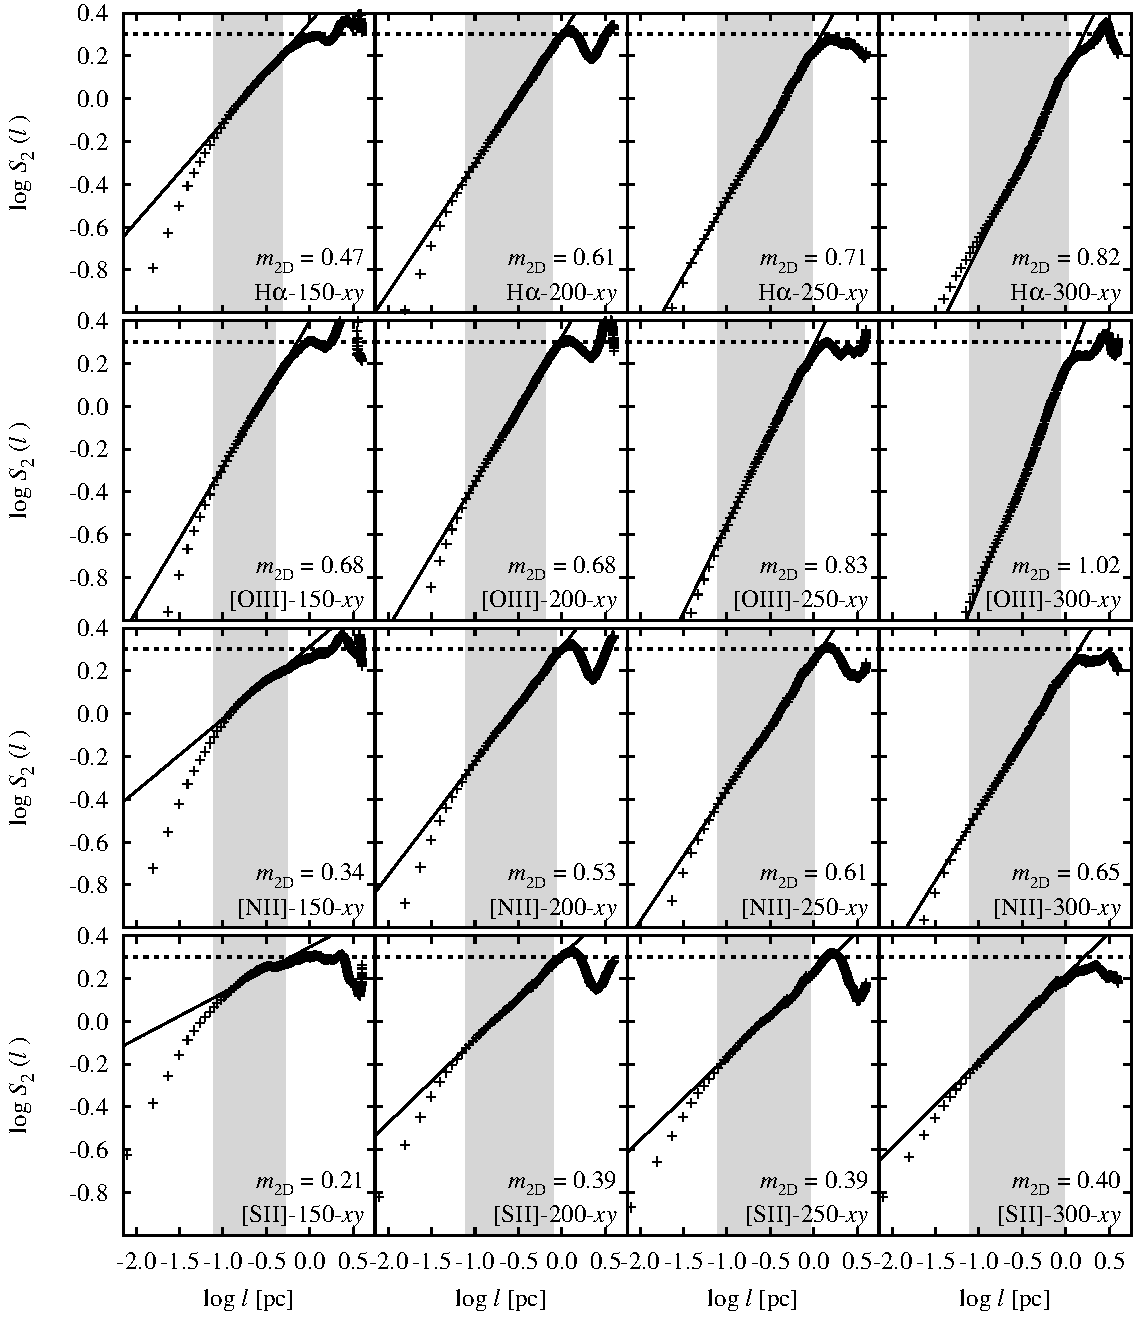
\includegraphics[width=\textwidth]{sf-all-xy-ref}
  \caption{Second-order structure functions against length scale for
    projection onto the $xy$-plane. From top to bottom: H$\alpha$,
    \oiii$\lambda 5007$, \nii$\lambda 6584$, \sii$\lambda 6716$. From
    left to right: 150,000, 200,000, 250,000 and 300,000~years. The
    points represent the calculated structure function for the
    numerical simulation. The solid line is the least-squares fit to
    the data points between limits described in the text, represented
    by the grey rectangle. The horizontal dotted line at $\log 2$ is
    included as a reference value.}
\label{fig:sfunc}
\end{figure*}
\begin{figure*}
 \centering
 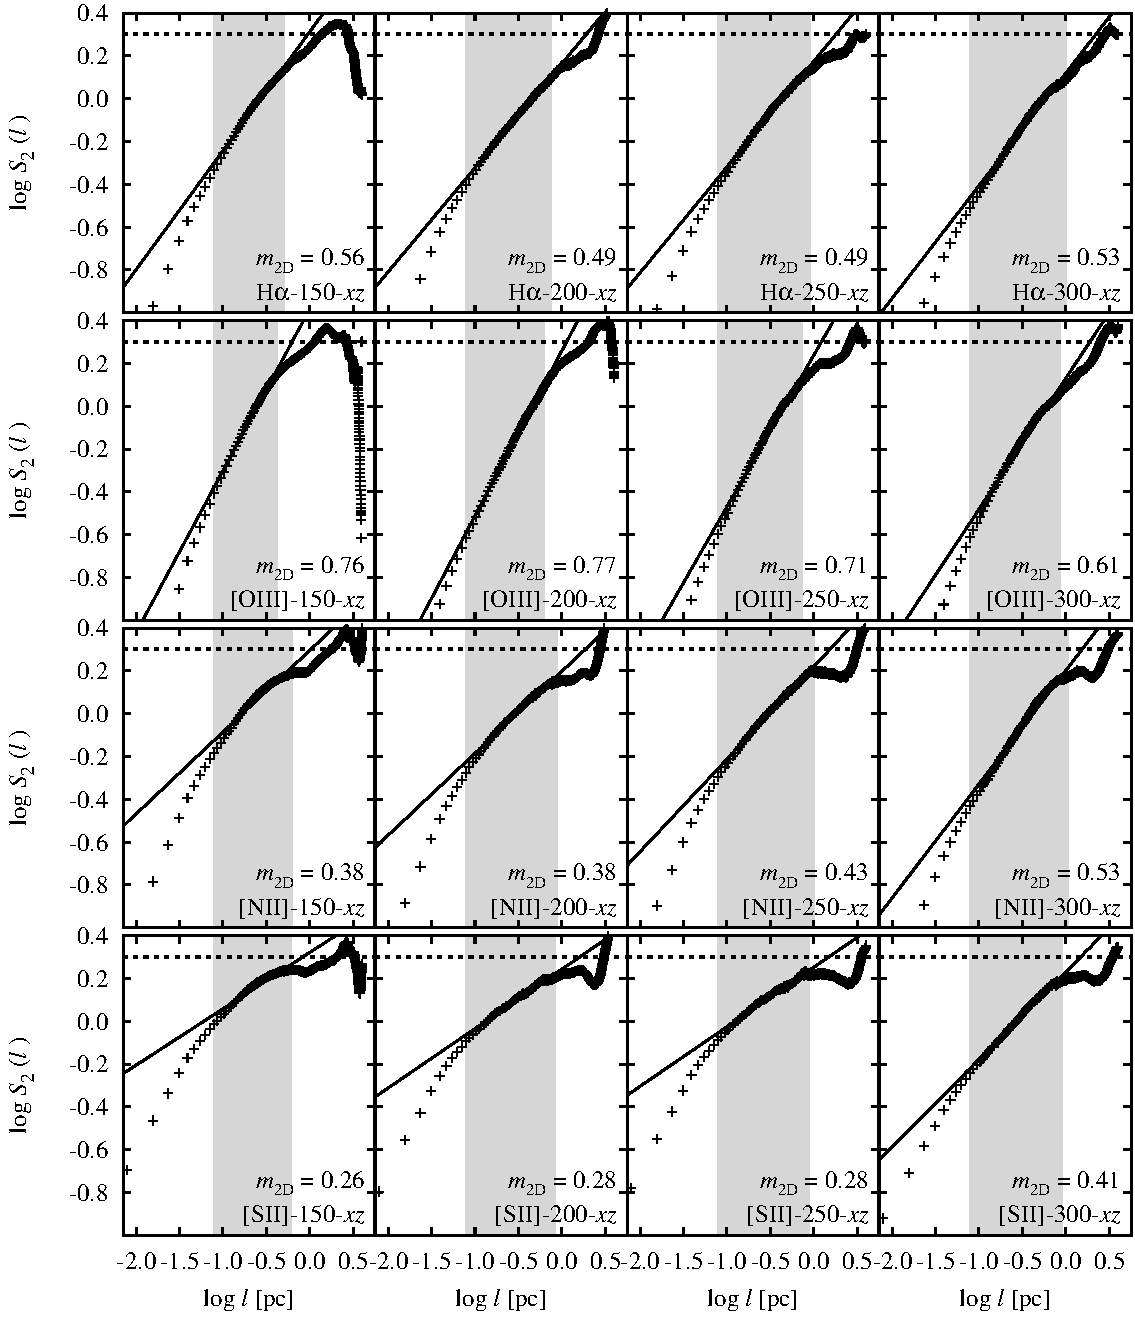
\includegraphics[width=\textwidth]{sf-all-xz-ref}
 \caption{Same as Fig.~\protect\ref{fig:sfunc} but for a projection
   onto the $xz$ plane.}
 \label{fig:sfuncxz}
\end{figure*}
\begin{figure*}
  \centering
  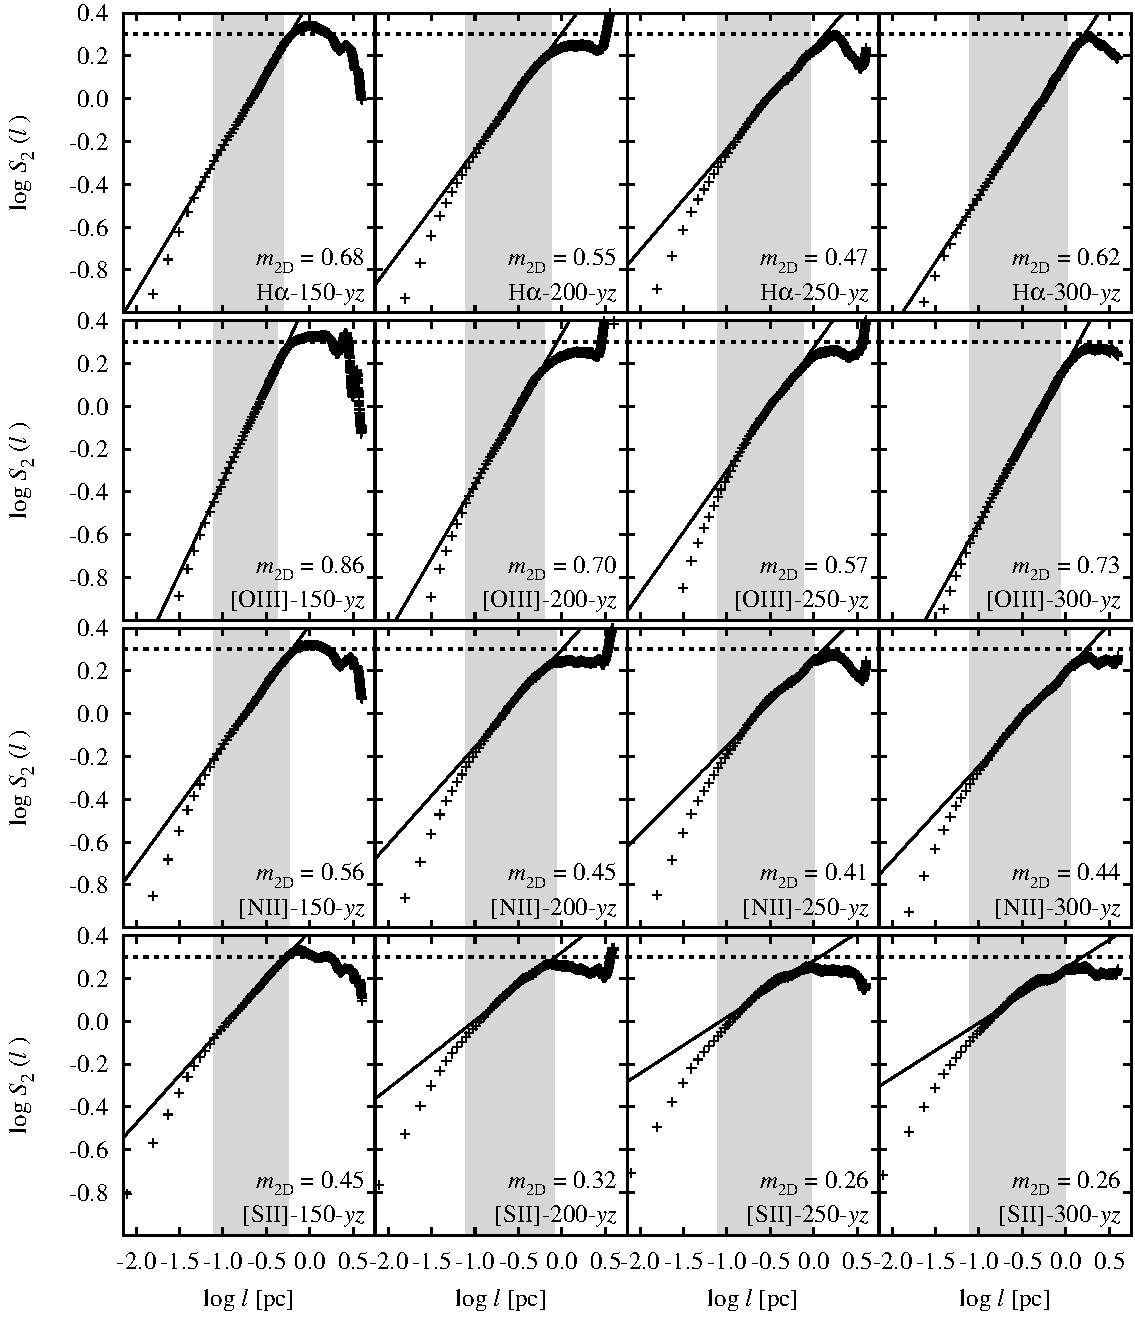
\includegraphics[width=\textwidth]{sf-all-yz-ref}
  \caption{Same as Fig.~\protect\ref{fig:sfunc} but for a projection
    onto the $yz$-plane.}
  \label{fig:sfuncyz}
\end{figure*}

\section[]{Example power spectra from Velocity Channel Analysis}
\label{app:vca}
Figures~\ref{fig:vca} to~\ref{fig:vcayz} show the power spectra
resulting from the velocity channel analysis (see
\S~\ref{sec:stats-vca}). Each of the three figures is for a different
viewing direction and shows the four emission lines at four different
times. For each combination of line and time, there are two panels: an
upper panel without including thermal Doppler broadening and a lower
panel with the broadening effects included.  In each graph, two power
spectra are plotted: one representing a very thick velocity slice
(i.e., encompassing all the emission) and the other averaged over thin
velocity slices of width $\delta v \sim 5$~km~s$^{-1}$.  Also shown
are the least-squares power-law fits to the thin and very thick slice
spectra and the range in wavenumber over which the fit is
calculated. This wavenumber range corresponds to the length-scale
range used for the structure function fits (see
\S~\ref{sssec:s2func}).  The very thick velocity slice is equivalent
to the total intensity along the line of sight and its power spectrum
does not vary with the addition of thermal broadening.

It is clear that the thermal broadening has a large effect on the VCA
of the H$\alpha$ line, effectively erasing the difference in slope
between the thin and thick slices.  For photoionized gas at $T_e=
10^4$~K, the FWHM of the H$\alpha$ line is $\sim 22$~km~s$^{-1}$,
while that of an oxygen line is a quarter of this, $\sim
5.5$~km~s$^{-1}$.  Indeed, the heavier ions are less affected by thermal broadening, but a slight steepening of the thin-slice power spectra can still be seen, amounting to a reduction in \gammaVCAthin{} of \(\sim 0.1\). 

For the thermally broadened case, the variation with time of the
slopes of these fits, \gammaVCAvthick{} for the thick slices and
\gammaVCAthin{} for the thin slices, is shown in
Fig~\ref{fig:vcatrends} and discussed in \S~\ref{sssec:vca}.

\end{document}
